\chapter{Checks concerning the enhancement at low \Dz\proton mass}
\label{sec:Structure}

In section \ref{sec:Signalfit} it has been stated that the fit of the \Dz\proton mass spectrum needs an additional component to parametrize an enhancement at low \Dz\proton masses right after threshold.
An appropriate model for that enhancement has seemed to be parametrized like the two \LcResI and \LcResII resonances.
This doesn't mean at all that there is really an additional resonance seen.
There might be a lot of other reasons, e.g.:
\begin{itemize}
    \item Detector threshold / acceptance effects,
    \item Low mass behaviour induced by some selection requirements,
    \item Feed-down from partially reconstructed decays,
    \item Threshold enhancement due to wide resonances below \Dz\proton mass threshold.
\end{itemize}
In this chapter several checks are done to either explain the origin of this enhancement or rule out some of the ideas.
It should be mentioned, that there won't be a final answer to that question.
If this was really something new, it would be really hard to prove it with a semileptonic decay channel.
There is currently another \lhcb analysis on the exclusive hadronic decay \decay{\Lb}{\Dz\proton\pim} running, seeing a similar enhancement at low \Dz\proton mass.
This channel enables to study the enhancement with more methods for instance with an amplitude analysis making it possible to tell more about it.

\section{Detector threshold / acceptance effect}
One possible explanation of the enhancement might be a simple threshold respectively acceptance effect of the detector or caused by the application of some selection requirements.
To clarify this possibility and estimate the effects of the detector and the selection requirements the simulation samples at generator level and at reconstruction level are used.
Figure \ref{fig:detector_cut_effect} shows the invariant \Dz\proton mass at different stages in generation and reconstruction.
The green distribution shows the \Dz\proton mass at generation level, i.e. there's no simulation of the detector or any reconstruction applied here.
In blue one sees the \Dz\proton mass after the simulation of the detector and in red the mass after reconstruction and selection.
For comparison the measured data distribution is shown in black as well.
In this case always the so called ``true" masses are plotted, i.e. there are no influences of the detector resolution in these distributions.
This figure shows that the distribution behaves similar and there isn't any significant acceptance effect arising neither due to the detector itself nor due to the reconstruction and selection process. 
Thus, the enhancement can't be caused by such an effect.
\begin{figure}[hptb]
	\centering
	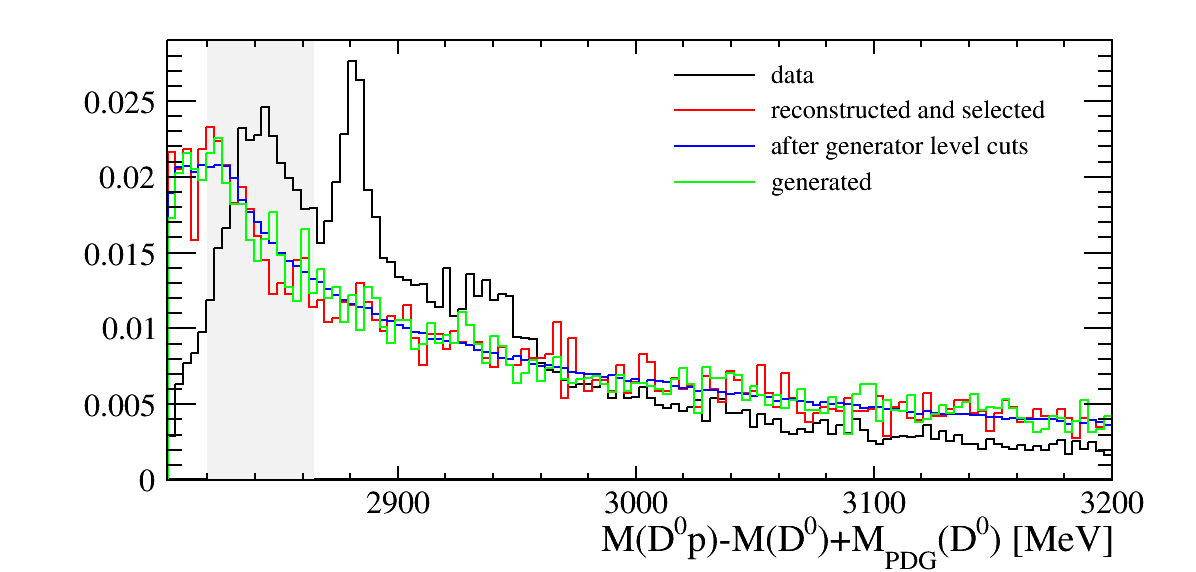
\includegraphics[width=0.49\textwidth]{LbToD0p/structure/detector_cut_effect}
	\caption{Simulated (true) invariant \Dz\proton mass at different stages, namely after generation (green), detector simulation (blue) and reconstruction and selection (red). The black line shows the measured data.}
	\label{fig:detector_cut_effect}
\end{figure}

Excluded to get any structure from acceptance effects a closer look at the \Dz\proton mass threshold reveals some kind of a ``S-shaped" curvature in the ascending part.
This can be better seen with a zoom into this region as shown in figure \ref{fig:mD0p_zoom}.
\begin{figure}[hptb]
	\centering
	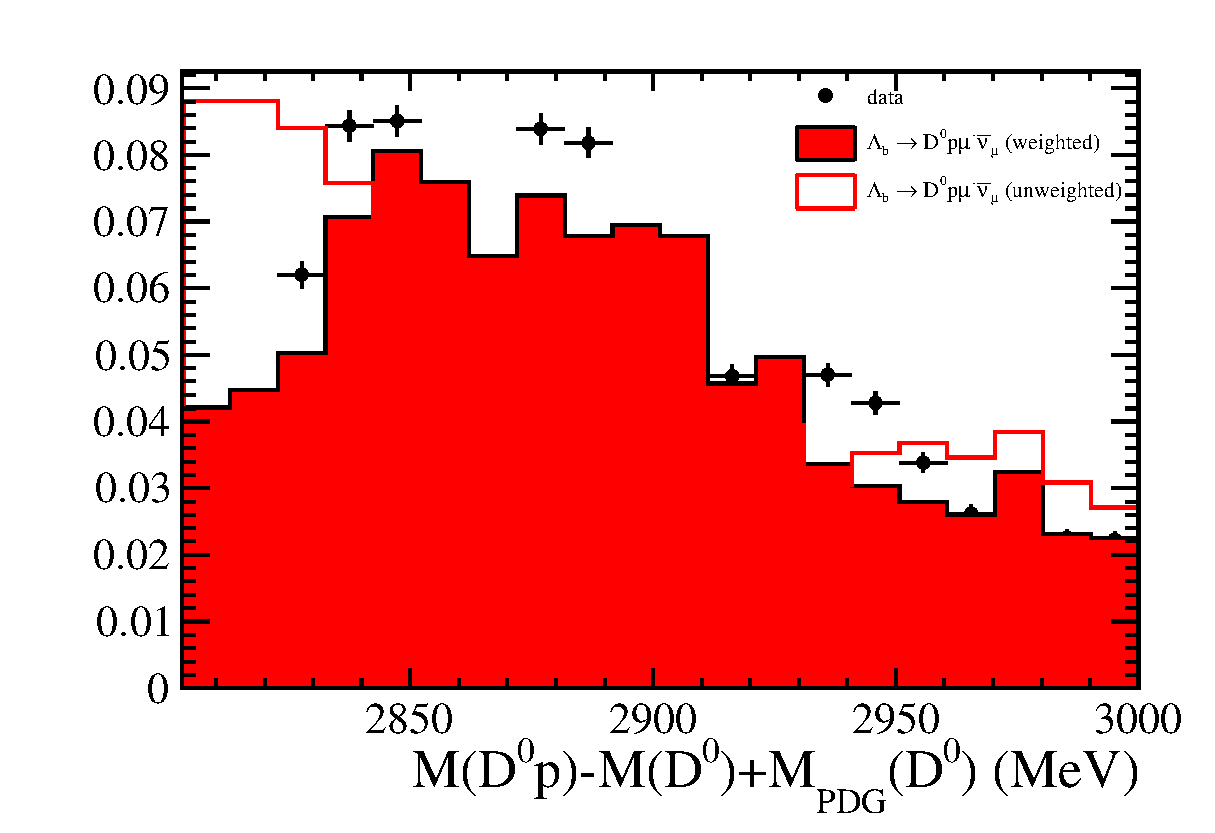
\includegraphics[width=0.49\textwidth]{LbToD0p/plots/data/Bh_DELTA_MASS_zoom}
	\caption{Zoom into the low \Dz\proton mass region.}
	\label{fig:mD0p_zoom}
\end{figure}

Due to this curvature the fit isn't able to describe the low \Dz\proton mass region only with a nonresonant component but rather prefers to have an additional component. 
At this point it should be mentioned that there are other analyses seeing a similar behaviour in this \Dz\proton mass region.

First of all, there is a study by \babar on the \Dz\proton final state (see fig. \ref{fig:Babar_D0p} aiming to measure the \LcResI and \LcResII resonance (and in the latter case to even observe it).
While discussing their systematics, they're wondering if this much less pronounced (compared to this analysis) bump at roughly 2840\mev might change their results by adding an additional resonance component to their fit. 
Since the impact isn't that large they just include the deviations in their systematics, unfortunately without trying to understand the origin of this bump \cite{BaBar_D0p}.
\begin{figure}[hptb]
	\centering
	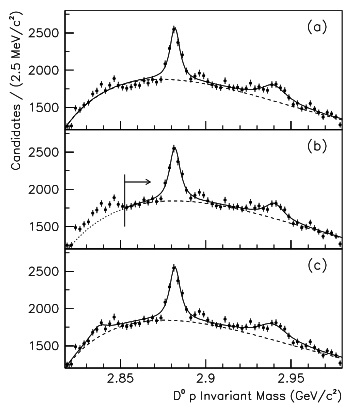
\includegraphics[width=0.49\textwidth]{Babar_D0p}
	\caption{\babar study on the \Dz\proton final state. They suspect to see a structure similar to the enhancement in the current analysis and fit it in c) with an additional resonance component for their systematic studies. Figure taken from \cite{BaBar_D0p}.}
	\label{fig:Babar_D0p}
\end{figure}

Furthermore, there are two more running \lhcb studies on either prompt \Dz\proton events and on the hadronic \decay{\Lb}{\Dz\proton\pim} decay.
It can be disclosed that they are struggling with the same problem, seeing a pronounced enhancement around 2840\mev without being (currently) able to explain it.
However, since there doesn't exist any approved material, nothing of their plots can be shown in this thesis.

Being seen in different channels and analyses substantiates the assumption, that there is a physical reason for the enhancement.

\section{Threshold enhancement from other resonances}
In principle it might be possible that resonances below the \Dz\proton mass threshold of 2803 \mev can enter the distribution due to their finite width.
If this was the case, one would rather expect a steep enhancement of the threshold region without having such a ``S-shaped" curvature.
Nonetheless there are two resonance candidates which might cause such a threshold enhancement and should be briefly discussed here.
There exists the broad \LcRes{(2765)} about which is hardly anything known.
Its width is currently quoted with 50 \mev in the PDG \cite{PDG}, but internal \lhcb measurements on \Lb form factors show that this is an overestimate of the \LcRes{(2765)} width.
The leakage into the \Dz\proton mass spectrum should thus be negligible.

Another resonance exactly sitting a the \Dz\proton mass threshold is the \SigmacpRes{(2800)}.
So far it is only seen in the hadronic decay \decay{\SigmacpRes{(2800)}}{\Lc\piz}, but the decay \decay{\SigmacpRes{(2800)}}{\Dz\proton} isn't forbidden by any conservation law\footnote{The quark content of the \SigmacpRes{(2800)} is (\uquark\dquark\cquark)}.
The mean mass of the \SigmacpRes{(2800)} with $2792^{+14}_{-5}\mev$ is indeed below the \Dz\proton mass threshold of 2803 \mev but it has a width of $62^{+60}_{-40}\mev$ \cite{PDG} and is thus a possible candidate for a threshold enhancement.
The \SigmacpRes{(2800)} itself could come from the decay \decay{\Lb}{\SigmacpRes{(2800)}\mun\neumb}, which hasn't been observed yet either.
It is thus hard to estimate how probable a threshold enhancement by this \SigmacpRes{(2800)} is.

\section{Possible background sources}
It has to be checked that the peaking structure of the enhancement isn't caused by any kind of background.
One can easily exclude that combinatorial background causes the enhancement.
First, it doesn't appear in the wrong sign \Dz\proton mass distribution as already shown in Figure \ref{fig:fit_WS}.
Second, a twodimensional plot of the invariant \Dz\proton mass versus \logIP distribution shows that the enhancement obeys the same line structure over \logIP than the \LcResI and \LcResII resonances (see Figure \ref{fig:plot_M_vs_logIP}).
This means that the decay topology looks exactly the same for the enhancement and the resonances leading to the conclusion that the enhancement looks like signal.
\begin{figure}[hptb]
	\centering
	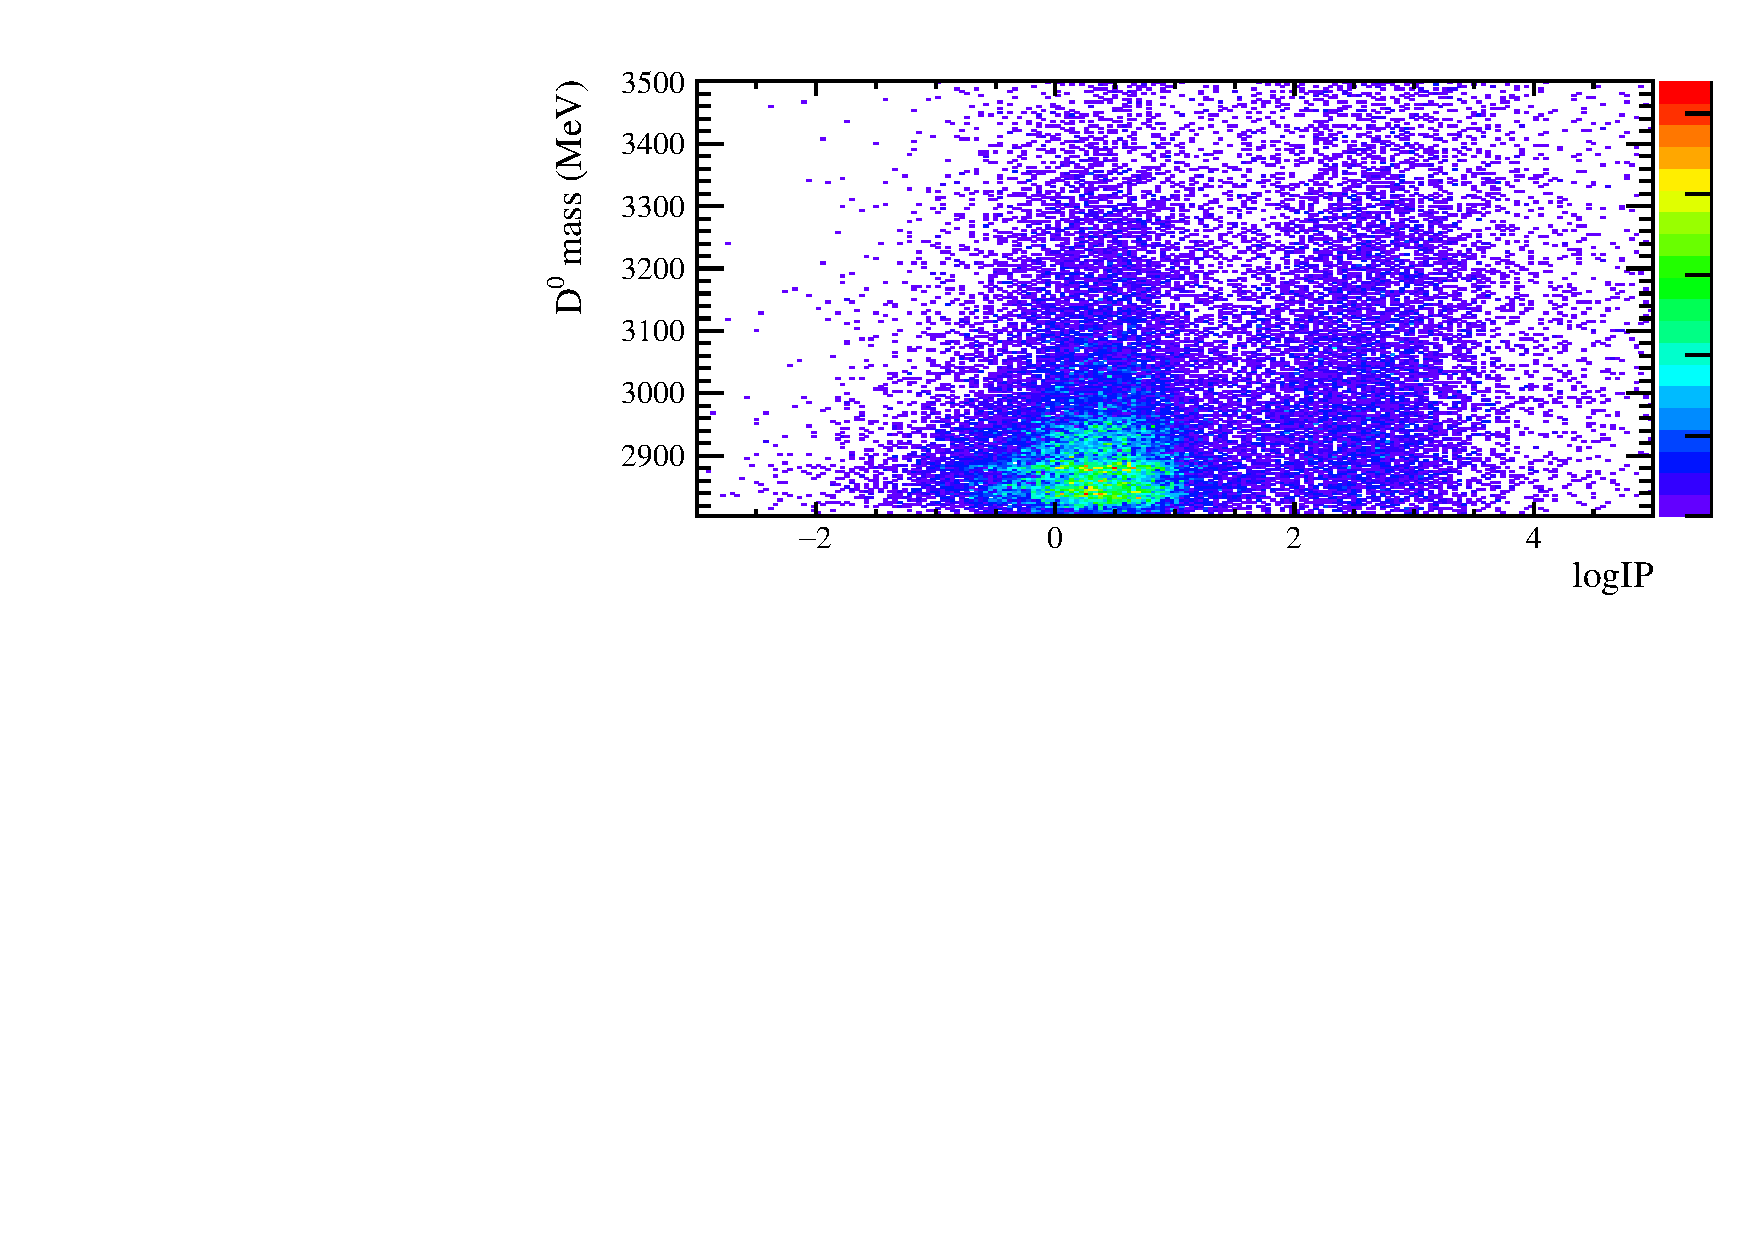
\includegraphics[width=0.49\textwidth]{LbToD0p/plots/data/M_vs_logIP_200Bins_RS}
	\caption{Invariant \Dz\proton mass versus \logIP distribution. The \LcResI and \LcResII are clearly visible as bands in \Dz\proton mass tending to cluster around $\logIP \approx 1$. The observed enhancement behaves very similar compared to the resonances excluding that the enhancement can't be caused by combinatorial backgrounds.}
	\label{fig:plot_M_vs_logIP}
\end{figure}

Albeit, Peaking backgrounds could enter the \Dz\proton mass spectrum due to either a misidentified \Dz or \proton.
For this purpose the invariant \Dz\proton mass is plotted for the \Dz mass sidebands, namely for events with $M(\Dz) < 1820 \mev$ or $M(\Dz) > 1910 \mev$.
As these events are clearly away from the \Dz mass peak, they have to be background.
Figure \ref{fig:plot_mD0p_mD0Sideband} shows that neither the enhancement nor any of the identified \Lc resonances appears here.
This is a clear sign, that backgrounds from fake \Dz don't cause the enhancement.
\begin{figure}[hptb]
	\centering
	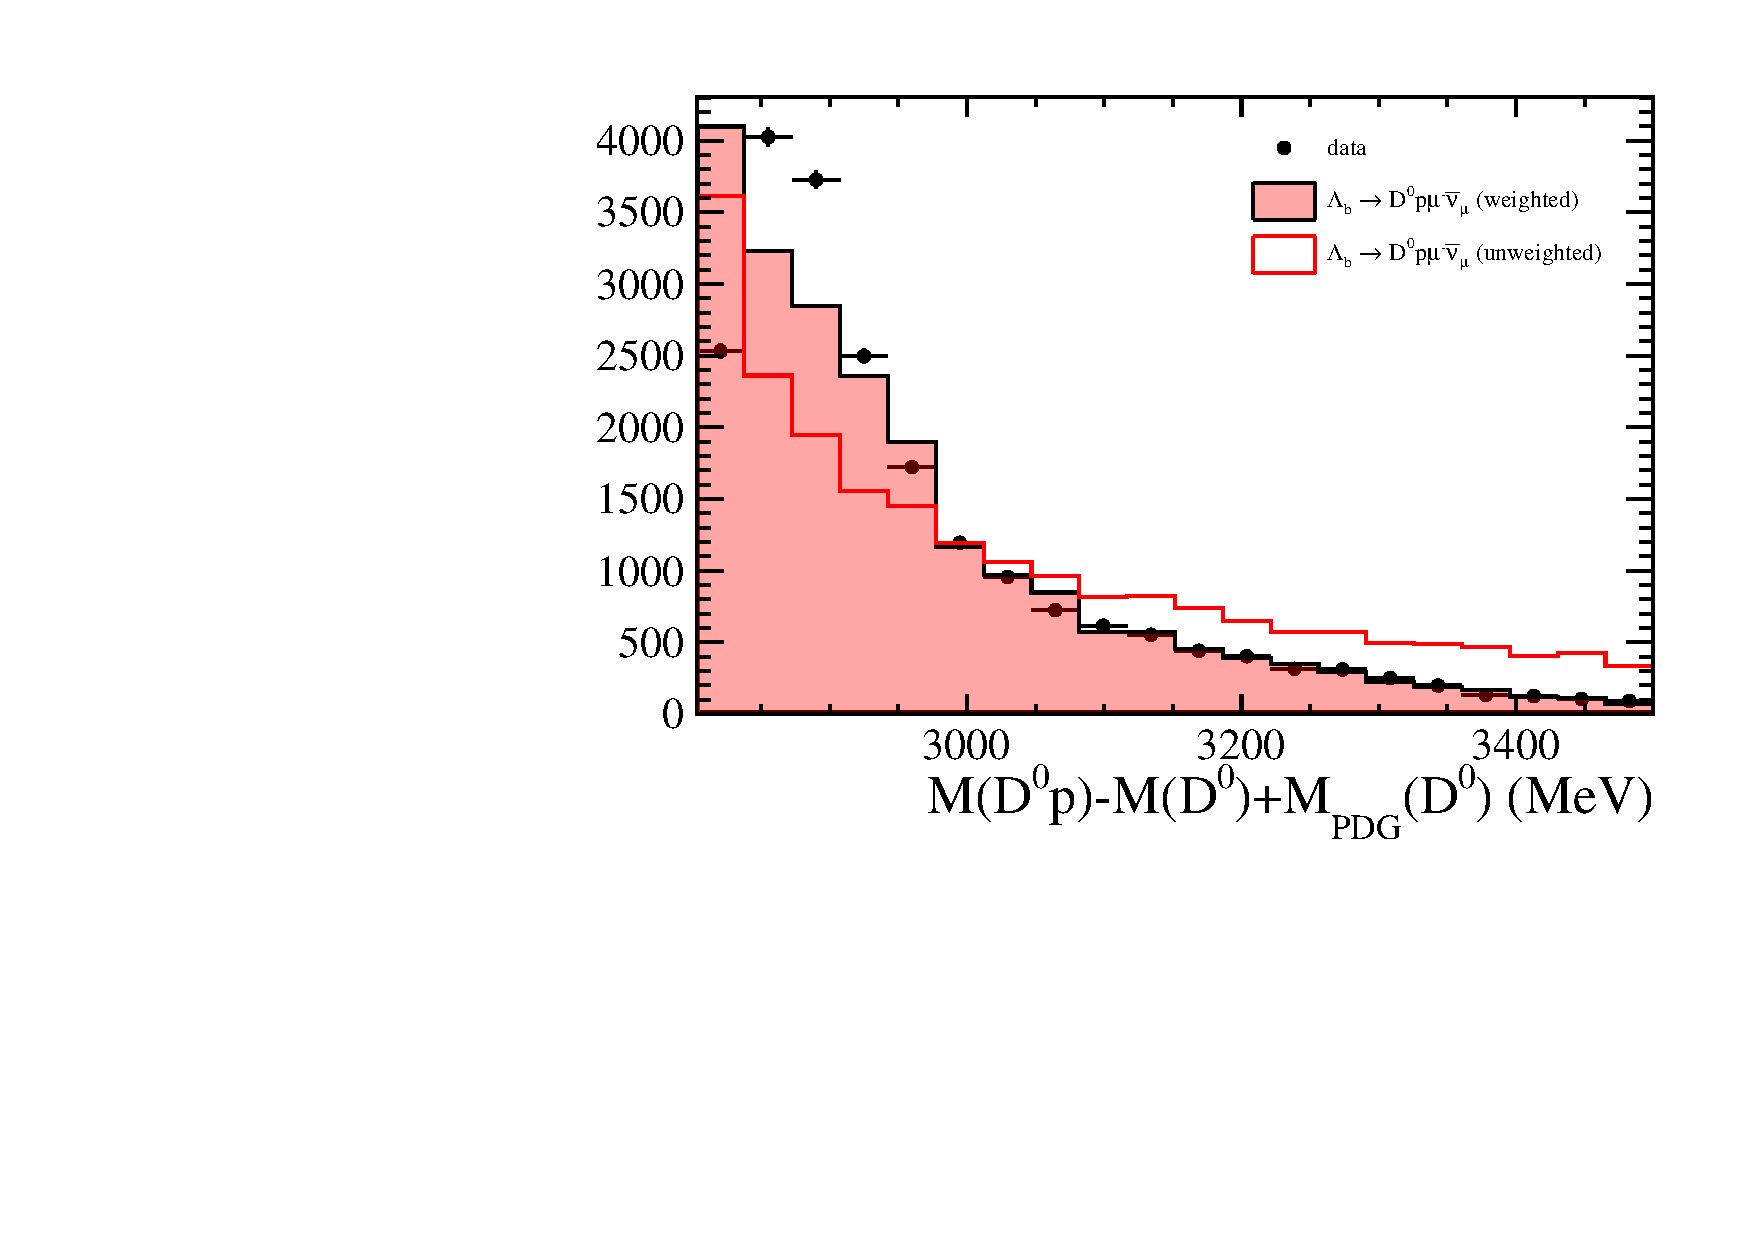
\includegraphics[width=0.49\textwidth]{LbToD0p/plots/data/Bh_DELTA_MASS_mD0Sideband}
	\caption{Invariant \Dz\proton mass for events in the \Dz mass sidebands $M(\Dz) < 1820 \mev$ or $M(\Dz) > 1910 \mev$. No enhancement or any other peaking structure can be seen, indicating that fake \Dz backgrounds don't cause the enhancement.}
	\label{fig:plot_mD0p_mD0Sideband}
\end{figure}

It is left to check for fake protons.
When estimating the amount of fake protons in section \ref{sec:BKG_misIDp} only an average value for the total misidentification ratio has been given.
However, it is conceivable, that the misidentification ratio depends on the \Dz\proton mass and is particularly high in the enhancement region.
Thus, the estimate of the misidentification ratio is repeated for three bins in \Dz\proton mass to see if fake protons are more likely to be in the enhancement region.
One obtains for the misidentification ratio:
\begin{itemize}
    \item $(\misIDratiobinIval \pm \misIDratiobinIerr)\%$ for $\MDp < 2860 \mev$,
    \item $(\misIDratiobinIIval \pm \misIDratiobinIIerr)\%$ for $2860 < \MDp < 3000 \mev$,
    \item $(\misIDratiobinIIIval \pm \misIDratiobinIIIerr)\%$ for $\MDp > 3000 \mev$.
\end{itemize}
The bins have been chosen such that the first one only covers the enhancement region, the second bin the \LcResI and \LcResII resonances and the third bin the region above.
Interestingly, the misidentification ratio is the smallest in the enhancement region.
It is the region with least pollution from fake backgrounds.
As further crosscheck can be seen in Figure \ref{fig:plot_mD0p_PIDcuts}. 
Here, the invariant \Dz\proton mass is plotted for different tight requirements on the particle identification (PIDp and PIDp$-$PIDK) of the proton.
All other requirements are the same as described in section \ref{sec:Selection}.
If the enhancement is made up of events with particles misidentified as protons, then it should disappear if one tightens the requirements on the proton identification.
However, this isn't the case here.
The enhancement stays as pronounced as the \LcResI resonance for increasing PIDp and PIDp$-$PIDK variables and should thus be made up of real protons.
\begin{figure}[hptb]
	\centering
	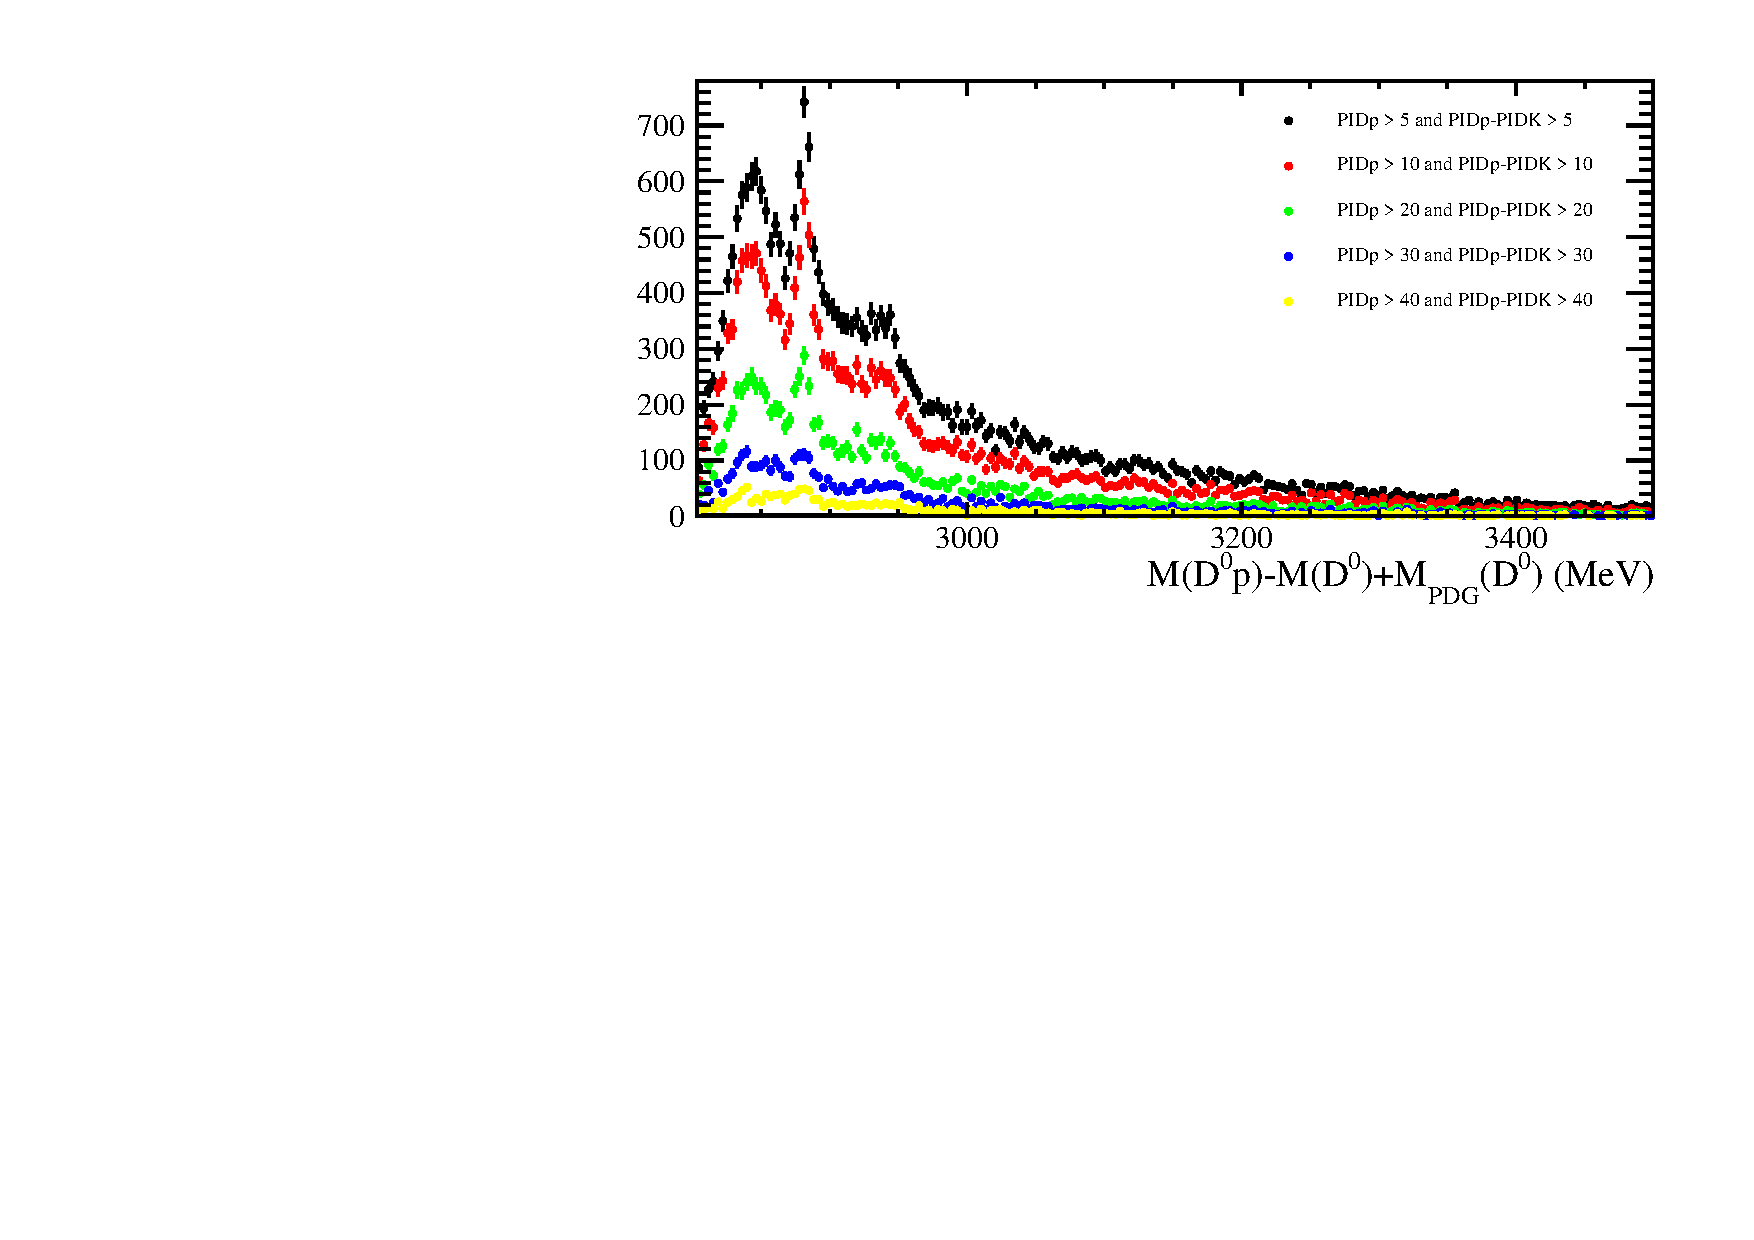
\includegraphics[width=0.49\textwidth]{LbToD0p/structure/mD0p_PIDcuts}
	\caption{Invariant \Dz\proton mass for different requirements on the proton's particle identification variables PIDp and PIDp$-$PIDK (for a definition of these variables see section \ref{sec:Selection}). 
             The enhancement doesn't disappear with tighter requirements on the proton identification.
             This confirms that real protons make up the enhancement.
    }
	\label{fig:plot_mD0p_PIDcuts}
\end{figure}

\section{Partially reconstructed decays}
Assuming that real protons and \Dz cause the enhancement it isn't said that this enhancement is a resonance decaying into a \Dz\proton.
It might be that one sees a so called ``feed down" from a partial reconstructed decay.
Partial reconstructed decay means that not all particles participating in an event are reconstructed.
A good example are semileptonic decays like \LbToDpmunuX since the neutrino isn't reconstructed.
This is furthermore an inclusive measurement, i.e. there might some unknown particles $X$, which is another example for not reconstructing all particles.
Another issue at \lhcb is, that pions aren't often reconstructed and thus missing.
One possibility of getting a peak in \Dz\proton mass without being a direct decay product would be that the inital \Lb decays semileptonically into some resonance $R$ and this resonance $R$ afterwards decays into a \Dstar\proton.
The \Dstar decays into a \D\pion in turn.
The total decay chain would then be \decay{\Lb}{R\mun\neumb}, \decay{R}{\Dstar\proton} and \decay{\Dstar}{\D\pion}.
If one misses the final state \pion and combines the \D and the \proton to look at the invariant \D\proton mass, a peak appears here, which isn't the product of a resonant decay \decay{\tilde{R}}{\D\proton}, but rather just the ``reflection" or ``feed-down" from a different decay of another
resonance $R$.
To check if the enhancement is a feed-down from a different decay and a potentially well-known resonance a tool recently developed by Marian Stahl, a Heidelberg Ph.D. student, is used.
It enables to isolate tracks, i.e. it is possible to require and control, how many tracks come from a certain decay vertex.
With this ability two further plots of the \Dz\proton invariant mass are produced and plotted in Figure \ref{fig:mD0p_AdditionalParticles}:
The left one shows the invariant \Dz\proton mass distribution requiring that no other charged hadron (e.g. \pion, \kaon) comes from the \Dz\proton\mun decay vertex.
This means that this plot should show \Lb decays into \Dz\proton\mun without any other charged particles.
Since neutral particles don't leave tracks in the detector, there could be some neutral particles, still.
The well known \Dz\proton spectrum can be seen there including the resonances \LcResI and \LcResII as well as the enhancement.
In the right plot of Figure \ref{fig:mD0p_AdditionalParticles} it is required that there is at least one additional charged particle coming from the \Dz\proton\mun decay vertex.
Following this, it shows the invariant \Dz\proton mass distribution for partially reconstructed decays.
The \LcResI, \LcResII resonances as well as the enhancement have vanished.
This is a clear sign, that the enhancement likely decays into \Dz\proton and is not an effect of partial reconstructed decays.
\begin{figure}[hptb]
	\centering
	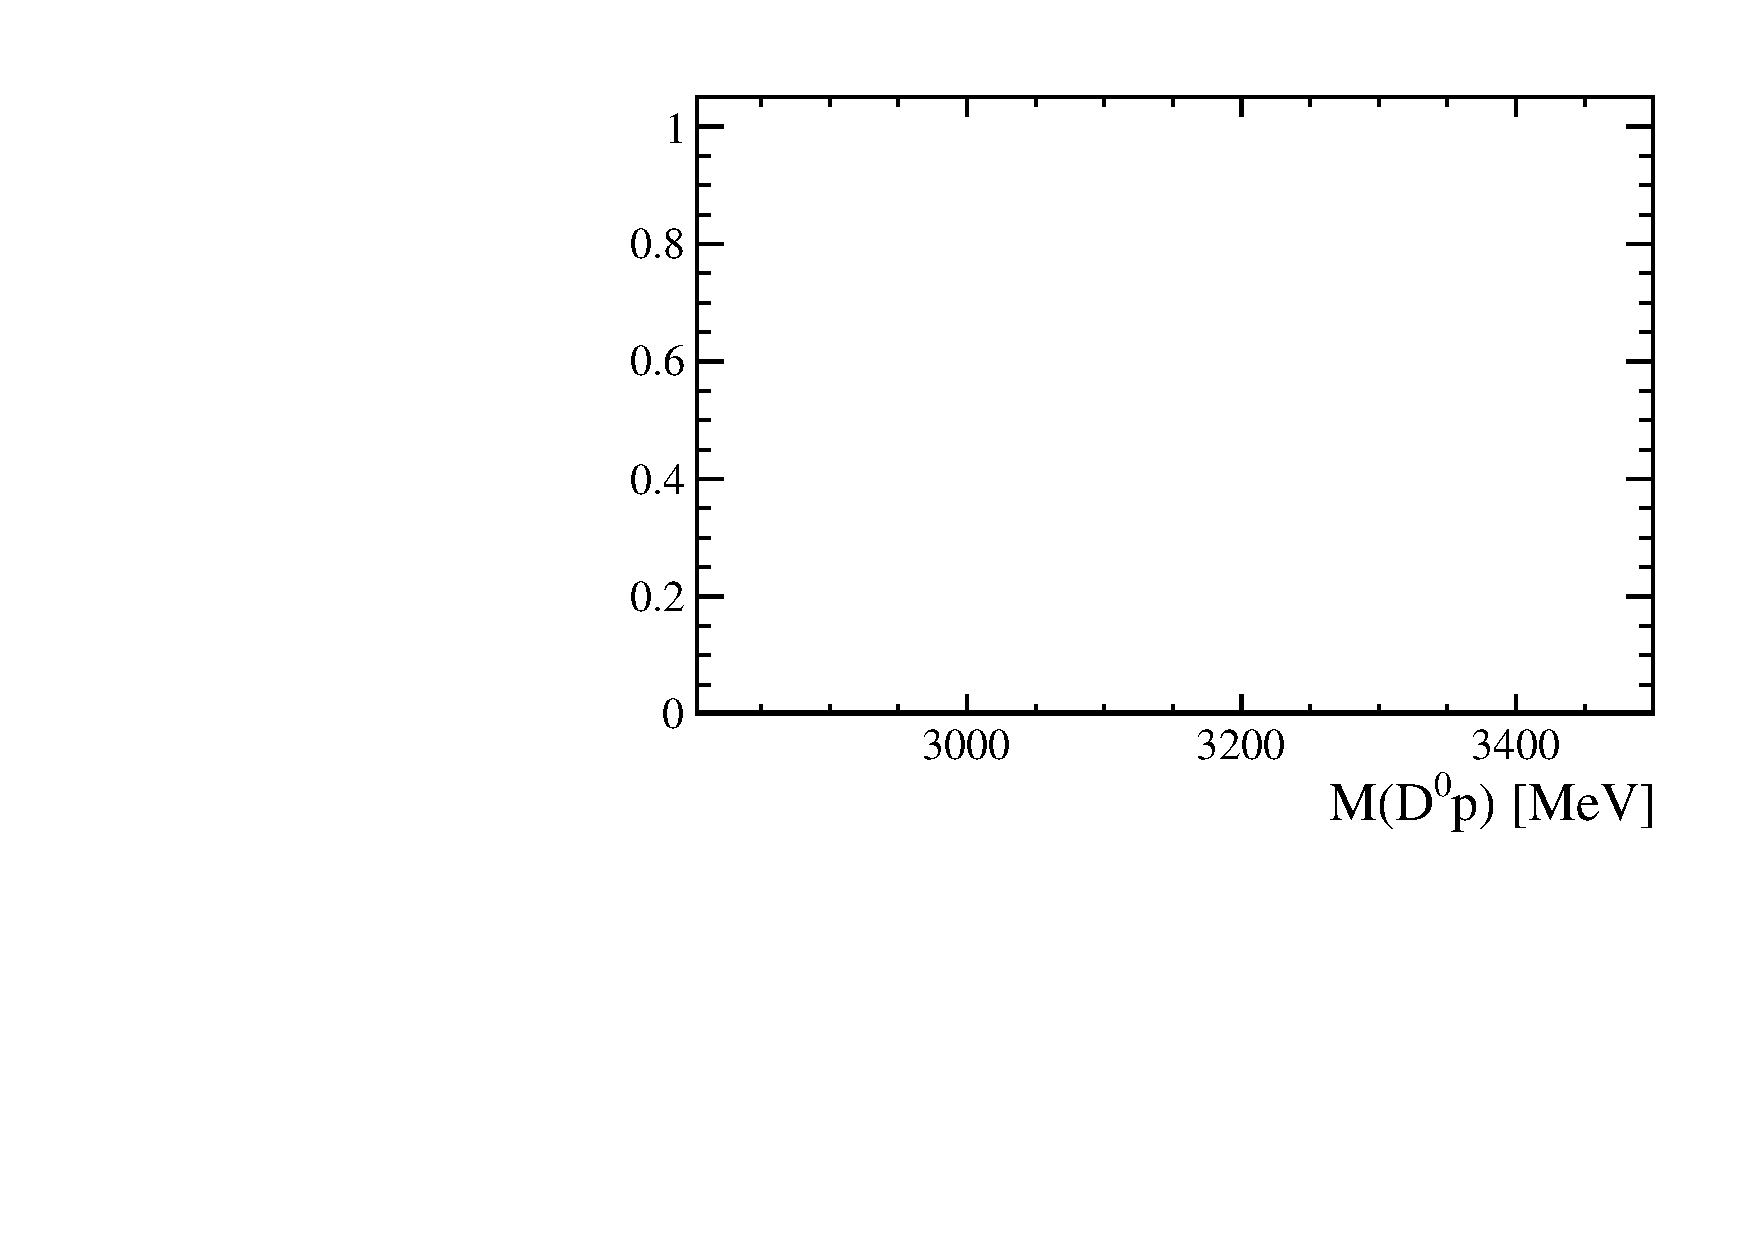
\includegraphics[width=0.49\textwidth]{LbToD0p/TupleToolPlots/mD0p}
	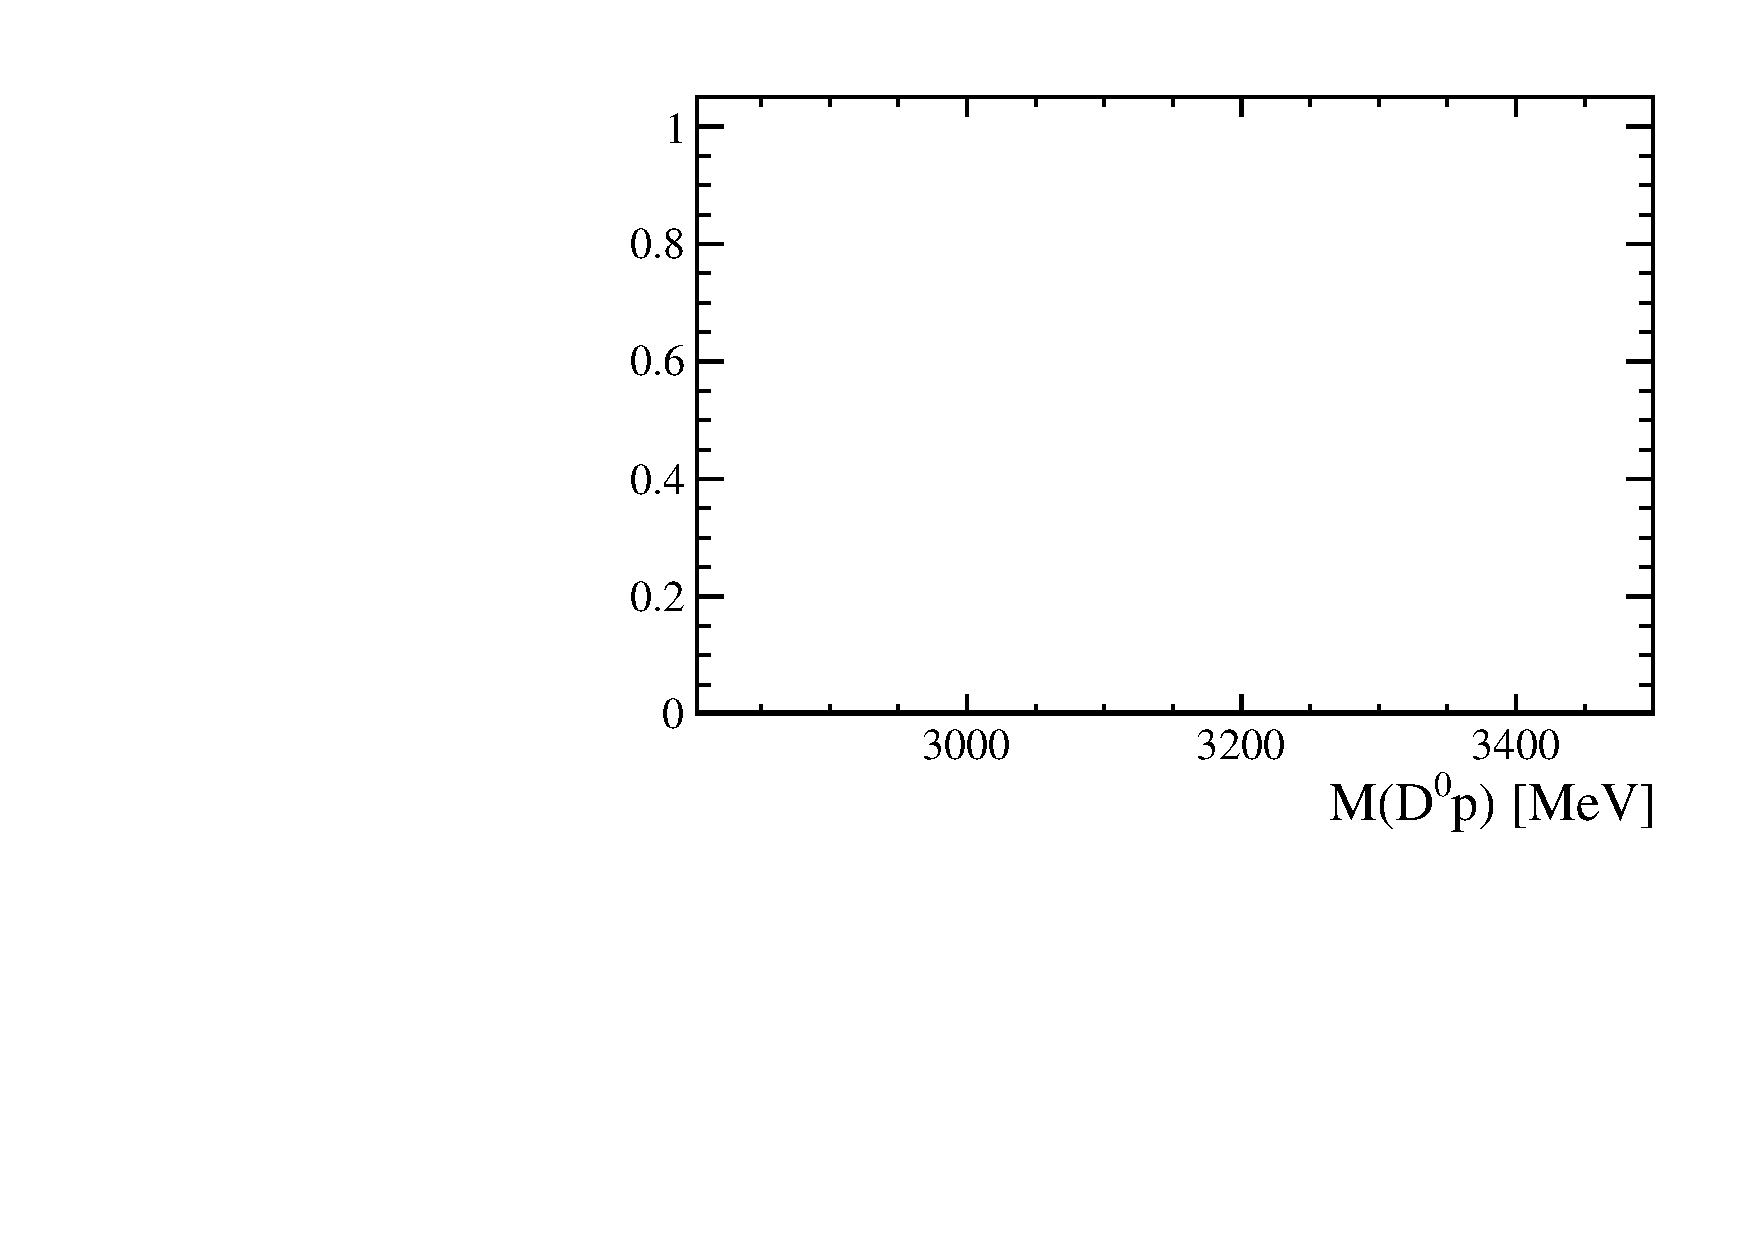
\includegraphics[width=0.49\textwidth]{LbToD0p/TupleToolPlots/mD0p_AddedParticles}
	\caption{Invariant \Dz\proton mass where no other (charged) hadron leaves the \Dz\proton\mun decay vertex (left) and with at least on additional hadron coming from the \Dz\proton\mun decay vertex.
             In the first case the \LcResI and \LcResII resonance as well as the enhancement are clearly visible.
             In the latter case with additional hadrons, the peaking structure and above all the enhancement vanishes. 
             As a consequence it is very probable that the enhancement originates from direct decays into \Dz\proton.
    }
	\label{fig:plot_mD0p_AdditionalParticles}
\end{figure}

It should again noted, that it is hard to conclude anything for additional neutral particles since they don't leave a track in the detector.
Having \D mesons in a mass spectrum, it is very common that one sees peaks coming from a partially reconstructed decay with a \decay{\Dstar}{\D\pion}.
As a last check a possible impact on the \Dz\proton mass spectrum for the special case of a \decay{\Dstarz}{\Dz\piz} decay with mising the \piz is estimated:
Assuming that there exists a resonance $R^{+}$, obeying the decay chain \decay{\Lb}{R^{+}\mun\neumb}, \decay{R^{+}}{\Dstarz\proton} and \decay{\Dstarz}{\Dz\piz}, the question comes up, which mass this resonance $R^{+}$ must have, to cause a peak in \Dz\proton mass in the enhancement region.
A simple phase space simulation delivers that this mass of $R^{+}$ should be about $2980\mev$.
Indeed, there exists a resonance, namely the \XicpRes{(2980)} with a mass of $(2971 \pm 3.3)\mev$ \cite{PDG}.
However, the quark content of a \Xicp is (\uquark\cquark\squark) whereas neither a \Dstarz nor the proton contain a \squark quark.
Thus, the decay \decay{\XicpRes{(2980)}}{\Dstarz\proton} would need to go through the weak interaction.
Nonetheless the \XicpRes{(2980)} is heavy enough to decay also hadronically. 
That's why the potential decay \decay{\XicpRes{(2980)}}{\Dstarz\proton} is highly suppressed.
So there is currently no resonance known that can decay via a \Dstarz\proton and have a mass that allows to peak in the \Dz\proton mass.

\section{General conclusions on the enhancement}
In the previous sections different attempts have been made to find either a solution or rule out some potantial explanations of the enhancement seen in the invariant \Dz\proton mass spectrum of the \LbToDpmunuX channel.
An effect from the detector as well as backgrounds especially from misidentified particles seem to be very unlikely.
By all indications there are real \Dz and protons involved in the nature of the enhancement.
It is likely that the process responsible for the enhancement is directly decaying into a \Dz\proton final state without being a ``feed-down" from a partially reconstructed decay, whereas the presence of neutral particles can't be ruled out.
Finally it can't be concluded if there is a new resonance appearing in the invariant \Dz\proton mass spectrum.
If this enhancement would we a new \Lc resonance then it should be seen in the \Lc\pip\pim final state as well, which isn't the case \cite{PDG}.
The question on the origin of the enhancement is still open and interesting to pursue.
One has to keep in mind that the main purpose of this thesis is the measurement of the inclusive branching ratio \BR(\LbToDpmunuX). 
Considering the fact that a lot of potential background sources causing the enhancement can be ruled out and the \Dz and proton seems to be involved in the enhancement, it seems to be justified that the yield of the enhancement is counted as signal to
the total signal yield \NDp in the nominal fit (see Section \ref{sec:Signalfit}). 
